\documentclass[12pt,a4paper]{report}

% --- Paquetes de Idioma y Codificación ---
\usepackage[utf8]{inputenc}
\usepackage[T1]{fontenc}
\usepackage[spanish, es-tabla]{babel}

% --- Diseño de Página ---
\usepackage{geometry}
\geometry{top=2.5cm, bottom=2.5cm, left=3cm, right=3cm}

% --- Matemáticas y Símbolos ---
\usepackage{amsmath, amssymb, amsthm}

% --- Colores y Cajas ---
\usepackage[dvipsnames]{xcolor}
\usepackage[most]{tcolorbox}

% Caption

\usepackage{caption}

% Gráficos

\usepackage{graphicx}

% Espaciadora

\newcommand{\esp}{\vspace{0.5cm}}

% promedio

\newcommand{\prom}[1]{\left\langle #1 \right\rangle}

% ket

\newcommand{\ket}[1]{| #1 \rangle}

% bra

\newcommand{\bra}[1]{\langle #1 |}

% braket

\newcommand{\braket}[2]{\langle #1 | #2 \rangle}

% Bibliografía

\usepackage[style=apa, backend=biber]{biblatex} % Estilo APA
\addbibresource{biblio.bib} % Nombre de tu archivo .bib

% Configuración de cajas personalizadas
\newtcolorbox{importante}{
	colback=red!5!white,
	colframe=red!75!black,
	title=Importante,
	fonttitle=\bfseries
}

\newtcolorbox{nota}{
	colback=blue!5!white,
	colframe=blue!75!black,
	title=Nota,
	fonttitle=\bfseries
}

% Definición de la caja de bibliografía
\newtcolorbox{bibliografia}{
	colback=gray!5!white,
	colframe=gray!75!black,
	title=Bibliografías útiles,
	fonttitle=\bfseries,
	breakable
}

% Socrative para óptica 2

\newtcolorbox{Socrative}{
	colback=orange!5!white,
	colframe=orange!75!black,
	title=Socrative,
	fonttitle=\bfseries,
	breakable
}

% Float

\usepackage{float}

% --- Hipervínculos ---
\usepackage{hyperref}
\hypersetup{
	colorlinks=true,
	linkcolor=blue,
	filecolor=magenta,      
	urlcolor=cyan,
}

% --- Datos del Documento ---
\title{Electromagnetismo}
\author{Chengyu Jin}
\date{\today}

\begin{document}
	
	\maketitle
	
	\tableofcontents
	\newpage
	
	\chapter{Campo magnético (magnetoestática $\partial B/\partial t = 0$) en la materia} 
	
	\section{Expansión multipolar del potencial vector}
	
    \begin{nota}
    	Generalmente nos enfocaremos, pero también hay ejercicios donde no son espiras.
    \end{nota}
	
	Si desea una fórmula aproximada para el potencial vectorial de una distribución de corriente localizada, válida en puntos distantes, es necesaria una expansión multipolar. Recuerde: la idea de una expansión multipolar es escribir el potencial en forma de una serie de potencias en $1/r$, donde $r$ es la distancia al punto en cuestión (Fig. 5.51); si $r$ es lo suficientemente grande, la serie estará dominada por la contribución no nula más baja, y los términos de orden superior pueden ignorarse. Como se estableció anteriormente:
	
	\esp
	
	\begin{equation}
		\frac{1}{\mathfrak{r}} = \frac{1}{\sqrt{r^2 + (r')^2 - 2rr' \cos \alpha}} = \frac{1}{r} \sum_{n=0}^{\infty} \left( \frac{r'}{r} \right)^n P_n(\cos \alpha),
	\end{equation}
	
	\esp
	
	\noindent donde $\alpha$ es el ángulo entre $\mathbf{r}$ y $\mathbf{r}'$. En consecuencia, el potencial vectorial de un lazo de corriente se puede escribir como:
	
	\esp
	
	\begin{equation}
		\mathbf{A}(\mathbf{r}) = \frac{\mu_0 I}{4\pi} \oint \frac{1}{\mathfrak{r}} d\mathbf{l}' = \frac{\mu_0 I}{4\pi} \sum_{n=0}^{\infty} \frac{1}{r^{n+1}} \oint (r')^n P_n(\cos \alpha) d\mathbf{l}',
	\end{equation}
	
	\esp
	
	\noindent o, más explícitamente:
	
	\esp
	
	\begin{equation}
		\mathbf{A}(\mathbf{r}) = \frac{\mu_0 I}{4\pi} \left[ \frac{1}{r} \oint d\mathbf{l}' + \frac{1}{r^2} \oint r' \cos \alpha \, d\mathbf{l}' + \frac{1}{r^3} \oint (r')^2 \left( \frac{3}{2} \cos^2 \alpha - \frac{1}{2} \right) d\mathbf{l}' + \dots \right].
	\end{equation}
	
	\esp
	
	Al igual que en la expansión multipolar de $V$, llamamos al primer término (que va como $1/r$) el término \textbf{monopolar}, al segundo (que va como $1/r^2$) \textbf{dipolar}, al tercero \textbf{cuadrupolar}, y así sucesivamente.
	
	\esp
	
	Ahora bien, el \textbf{término monopolar magnético es siempre cero}, ya que la integral es simplemente el desplazamiento vectorial total alrededor de un lazo cerrado:
	
	\esp
	
	\begin{equation}
		\oint d\mathbf{l}' = \mathbf{0}
	\end{equation}
	
	\esp
	
	Esto refleja el hecho de que no existen monopolos magnéticos en la naturaleza (una suposición contenida en la ecuación de Maxwell $\nabla \cdot \mathbf{B} = 0$, sobre la cual se basa toda la teoría del potencial vectorial).
	
	\esp
	
	En ausencia de cualquier contribución monopolar, el término dominante es el \textbf{dipolo} (excepto en el raro caso en que este también se anule):
	
	\esp
	
	\begin{equation}
		\mathbf{A}_{\text{dip}}(\mathbf{r}) = \frac{\mu_0 I}{4\pi r^2} \oint r' \cos \alpha \, d\mathbf{l}' = \frac{\mu_0 I}{4\pi r^2} \oint (\mathbf{\hat{r}} \cdot \mathbf{r}') \, d\mathbf{l}'
	\end{equation}
	
	\esp
	
	Esta integral puede reescribirse de una forma más esclarecedora si invocamos la Ec. 1.108, con $\mathbf{c} = \mathbf{\hat{r}}$:
	
	\esp
	
	\begin{equation}
		\oint (\mathbf{\hat{r}} \cdot \mathbf{r}') \, d\mathbf{l}' = -\mathbf{\hat{r}} \times \int d\mathbf{a}'
	\end{equation}
	
	\esp
	
	\begin{nota}
		Hemos usado una versión del \textbf{Teorema de Stokes}. Particularicemos el Teorema para una función vectorial $\vec{v}$ que sea igual a un vector constante $\vec{C}$ por un escalar $T$, esto es $\vec{v}=\vec{C}T$. Aplicando el teorema tenemos
		
		\esp
		
		\begin{equation}
			\oint_L \vec{v} \cdot d\vec{l} = \int_S \nabla \times \vec{v} \cdot d\vec{S} = \int_S \nabla \times (\vec{C}T) \cdot d\vec{S} 
		\end{equation}
		
		\esp
		
		Desarrollando el rotacional $\nabla \times (\vec{C}T) = T \nabla \times \vec{C} - \vec{C}\ \times \nabla T$, donde el rotacional de la constante es 0. Sustituyendolo en la ecuación de arriba tenemos.
		
		\esp
		
		\begin{equation}
			\int_S \nabla \times (\vec{C}T) \cdot d\vec{S} = \int_S - \vec{C}\ \times (\nabla  T) \cdot d\vec{S} = \vec{C}\ \int_S d\vec{S} \times (\nabla T)
		\end{equation}
		
		\esp
		
		Hemos aplicado una propiedad del rotacional en el último paso de la ecuación anterior. Usando ahora también $a\times b = -b \times a$ tenemos
		
		\esp
		
		\begin{equation}
			\vec{C} \oint_L T d\vec{l} = - \vec{C}\ \int_S (\nabla T) \times d\vec{S} 
		\end{equation}
		
		\esp
		
		Entonces aplicando esto con $T=\vec{r} \cdot \vec{r}'$ y $\vec{C} = 1$ obtenemos,
		
		\esp
		
		\begin{equation}
			\oint_L (\vec{r} \cdot \vec{r}') d\vec{l}' = - \int_S (\nabla' (\vec{r} \cdot \vec{r}')) \times d\vec{S}'
		\end{equation}
		
		\esp
		
		Desarrollando el gradiente $\nabla (\vec{r} \cdot \vec{r}') = \vec{r} \times (\nabla' \times \vec{r}') + \vec{r}' \times (\nabla' \times \vec{r}) + (\vec{r}\cdot\nabla')\vec{r}' + (\vec{r}' \nabla')\vec{r}$, el único que sobrevive es $(\vec{r}\cdot\nabla')\vec{r}'$, que calculando vale $\vec{r}$, el resto de los términos se cancelan porque $\vec{r}$ no tiene prima, entonces aplicando $\nabla'$ es nulo, el rotacional de $r'$ es nulo también.
		
		\esp
		
		\begin{equation}
			\oint_L (\vec{r} \cdot \vec{r}') d\vec{l}' = - \int_S \vec{r} \times d\vec{S}'
		\end{equation}
		
		\esp
		
		Como $\vec{r}$ no tiene prima, lo puedo sacar fuera de la integral. Lo que nos queda de integral es lo que hemos definido como $\vec{a} = \int d\vec{a}$.
		
		\esp
		
		\begin{equation}
			\oint_L (\vec{r} \cdot \vec{r}') d\vec{l}' = - \vec{r} \times \int_S d\vec{S}' = - \vec{r} \times \vec{a}
		\end{equation}
	\end{nota}
	
	\esp
	
	\noindent Entonces,
	
	\esp
	
	\begin{equation}
		\mathbf{A}_{\text{dip}}(\mathbf{r}) = \frac{\mu_0}{4\pi} \frac{\mathbf{m} \times \mathbf{\hat{r}}}{r^2}
	\end{equation}
	
	\esp
	
	\noindent donde $\mathbf{m}$ es el \textbf{momento dipolar magnético}:
	
	\esp
	
	\begin{equation}
		\mathbf{m} \equiv I \int d\mathbf{a} = I\mathbf{a}
	\end{equation}
	
	\esp
	
	\begin{figure}[H]
		\centering
		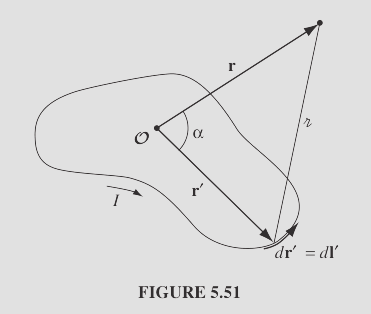
\includegraphics[width=0.5\textwidth]{IMG/fig551.png}
	\end{figure}
	
	\esp
	
	Aquí $\mathbf{a}$ es el ``\textbf{vector área}'' del lazo (Prob. 1.62); si el lazo es \textit{plano}, $\mathbf{a}$ es el área ordinaria encerrada, con la dirección asignada por la regla de la mano derecha habitual (dedos en la dirección de la corriente).
	
	\esp
	
	\noindent \textbf{Más cosas sobre $\vec{a}$}
	
	\esp
	
	\noindent En una superficie cerrada, $\vec{a}$ es nulo, esto es $\vec{a} = \oint_S d\vec{a} = 0$. 

	\esp
	
	\begin{nota}
		Al igual que antes, hemos usado el \textbf{Teorema de Divergencia}, pero también una versión, para el mismo caso de $\vec{v}$ vamos a aplicarlo en una superficie cerrada.
		
		\esp
		
		\begin{equation}
			\oint \vec{v} \cdot d\vec{S} = \int_v \nabla \cdot \vec{v} dV = \vec{C} \int_v (\nabla T) dV
		\end{equation}
		
		\esp
		
		donde hemos usado la propiedad $\nabla \cdot (\vec{C}T) = T \nabla \vec{C} + \vec{C} \nabla T$. Y el gradiente de la constante $\vec{C}$ es 0.
	\end{nota}
	
	\esp
	
	\noindent El momento dipolar magnético lo podemos expresar de la siguiente manera:
	
	\begin{equation}
		\vec{m} = I \vec{a} = \frac{1}{2} I \int \vec{r}' \times d\vec{l}'
	\end{equation}

	\esp
	
	Para ello usaremos la propiedad de $\oint d\vec{a} = 0$. Supongamos que una espira, al que podemos localizar con nuestro vector $\vec{r}'$ y $d\vec{l}'$ el vector que recorre la espira. Usamos el cono formado por los vectores anteriores, por lo que el borde sería la propia espira, ahora tomamos la superficie plano que define la propia espira, en realidad podemos usar cualquier otra superficie y nos daría lo mismo. Usando $\oint d\vec{a}=0$ tenemos.
	
	\esp
	
	\begin{equation}
		\oint_{total} d\vec{a} = \int_{cono} d\vec{a} + \int_{plano} d\vec{a} = 0 \implies \int_{plano} d\vec{a} = - \int_{cono} d\vec{a}
	\end{equation}

	\esp
	
	Cualquier superficie que tenga de borde la espira es equivalente a $-\int_{cono}d\vec{a}$. Resolviendo esta integral teniendo en cuenta que $d\vec{a}= (1/2) d\vec{r}\ '\times d\vec{l}'$ hemos demostrado lo que queríamos.
	
	\esp

	\noindent El campo magnético generado por el vector potencial debido al momento dipolar magnético es la siguiente
	
	\esp
	
	\begin{equation}
		\vec{B} = \nabla \times \vec{A} = \nabla \times \left( \frac{\mu_0 \vec{m}\times \vec{r}}{r^3} \right) = \frac{\mu_0}{4\pi} \left[ \frac{\nabla \times (\vec{m}\times\vec{r})}{r^3} + (\vec{m}\times\vec{r})\times\nabla\left(\frac{1}{r^3}\right) \right]
	\end{equation}
		
	\esp
	
	\noindent Desarrollando los rotacionales tenemos que $\nabla\times(\vec{m}\times\vec{r}) = 2\vec{m}$ y $\nabla\times(1/r^3)=-3\vec{r}/r^5$
	
	\esp
	
	\begin{equation}
		\vec{B} = \frac{\mu_0}{4\pi}\left( \frac{3(\vec{m}\cdot \vec{r})\vec{r}}{r^5} - \frac{\vec{mu}}{r^3} \right)
	\end{equation}
	
	\esp
	
	\begin{importante}
		$\vec{m}$ es independiente del origen de coordenadas, ya que el término monopolar es siempre nulo. La demostración es análogo para el caso del dipolar eléctrico.
	\end{importante}
	
	\esp
	
	Al igual que hicimos con el momento dipolar eléctrico puro, podemos definir un momento dipolar magnético puro cuando $\vec{a}\rightarrow 0$ y $I\rightarrow \infty$.
	
	\esp
	
	\noindent \textbf{EJERCICIO 3.37 apartado B HECHO EN RAW}
	
	\subsection{Fuerzas y pares de fuerzas sobre dipolos magnéticos}
	
	Un dipolo magnético experimenta un torque en un campo magnético, tal como lo hace un dipolo eléctrico en un campo eléctrico. Calculemos el torque sobre una espira de corriente rectangular en un campo uniforme $\mathbf{B}$. (Dado que cualquier espira de corriente puede construirse a partir de rectángulos infinitesimales, con todos los lados ``internos'' cancelándose, como se indica en la Fig. 6.1, no hay pérdida real de generalidad aquí; pero si prefiere empezar desde cero con una forma arbitraria, vea el Prob. 6.2). Centre la espira en el origen e inclínela un ángulo $\theta$ desde el eje $z$ hacia el eje $y$ (Fig. 6.2). 
	
	\esp
	
	\begin{figure}[H]
		\centering
		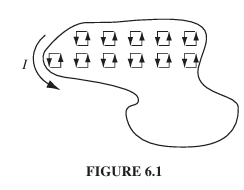
\includegraphics[width=0.5\textwidth]{IMG/fig61.png}
	\end{figure}
	
	\esp
	
	Sea $\mathbf{B}$ apuntando en la dirección $z$. Las fuerzas sobre los dos lados inclinados se cancelan (tienden a \textit{estirar} la espira, pero no la hacen \textit{rotar}). Las fuerzas en los lados ``horizontales'' son igualmente iguales y opuestas (por lo que la \textit{fuerza} neta sobre la espira es cero), pero sí generan un torque:
	
	\esp
	
	\begin{equation*}
		\mathbf{N} = aF \sin \theta \, \mathbf{\hat{x}}.
	\end{equation*}
	
	\esp
	
	La magnitud de la fuerza en cada uno de estos segmentos es
	
	\esp
	
	\begin{equation*}
		F = IbB,
	\end{equation*}
	
	\esp
	
	\noindent y por lo tanto
	
	\esp
	
	\begin{equation*}
		\mathbf{N} = IabB \sin \theta \, \mathbf{\hat{x}} = mB \sin \theta \, \mathbf{\hat{x}},
	\end{equation*}
	
	\esp
	
	\noindent o
	
	\esp
	
	\begin{equation}
		\boxed{\mathbf{N} = \mathbf{m} \times \mathbf{B}} \tag{6.1}
	\end{equation}
	
	\esp
	
	donde $m = Iab$ es el momento dipolar magnético de la espira. La Ecuación 6.1 da el torque sobre cualquier distribución de corriente localizada, en presencia de un campo \textit{uniforme}; en un campo \textit{no uniforme} es el torque exacto (respecto al centro) para un dipolo \textit{perfecto} de tamaño infinitesimal.
	
	\esp
	
	\begin{figure}[H]
		\centering
		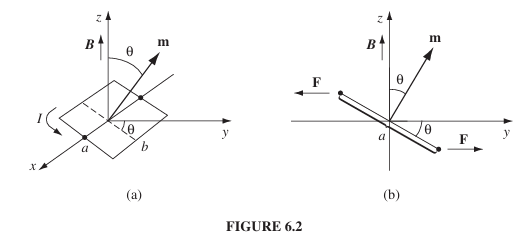
\includegraphics[width=0.7\textwidth]{IMG/fig62.png}
	\end{figure}

	\esp
	
	Note que la Ec. 6.1 es idéntica en forma al análogo eléctrico, la Ec. 4.4: $\mathbf{N} = \mathbf{p} \times \mathbf{E}$. En particular, el torque tiene nuevamente una dirección tal que alinea el dipolo \textit{paralelo} al campo. Es este torque el que explica el \textbf{paramagnetismo}. Dado que cada electrón constituye un dipolo magnético (imagínelo, si lo desea, como una pequeña esfera de carga en rotación), se podría esperar que el paramagnetismo fuera un fenómeno universal. En realidad, la mecánica cuántica (específicamente, el principio de exclusión de Pauli) tiende a agrupar a los electrones dentro de un átomo dado en pares con espines opuestos, y esto efectivamente neutraliza el torque sobre la combinación. Como resultado, el paramagnetismo ocurre con mayor frecuencia en átomos o moléculas con un número impar de electrones, donde el miembro ``extra'' desapareado está sujeto al torque magnético. Incluso aquí, la alineación está lejos de ser completa, ya que las colisiones térmicas aleatorias tienden a destruir el orden.
	
	\esp
	
	En un campo uniforme, la \textit{fuerza} neta sobre una espira de corriente es cero:
	
	\esp
	
	\begin{equation*}
		\mathbf{F} = I \oint (d\mathbf{l} \times \mathbf{B}) = I \left( \oint d\mathbf{l} \right) \times \mathbf{B} = \mathbf{0};
	\end{equation*}
	
	\esp
	
	\noindent la constante $\mathbf{B}$ sale de la integral, y el desplazamiento neto $\oint d\mathbf{l}$ alrededor de una espira cerrada se anula. En un campo \textit{no uniforme} este ya no es el caso. Por ejemplo, suponga que un anillo de alambre circular de radio $R$, que transporta una corriente $I$, está suspendido sobre un solenoide corto en la región de ``borde'' (Fig. 6.3). Aquí $\mathbf{B}$ tiene una componente radial, y existe una fuerza neta hacia abajo sobre la espira (Fig. 6.4):
	
	\esp
	
	\begin{equation}
		F = 2\pi I R B \cos \theta. \tag{6.2}
	\end{equation}
	
	\esp
	
	Para una espira \textit{infinitesimal}, con momento dipolar $\mathbf{m}$, en un campo $\mathbf{B}$, la fuerza es
	
	\esp
	
	\begin{equation}
		\boxed{\mathbf{F} = \nabla (\mathbf{m} \cdot \mathbf{B})} \tag{6.3}
	\end{equation}
	
	\esp
	
	\begin{figure}[H]
		\centering
		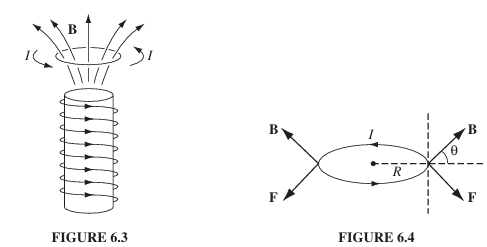
\includegraphics[width=0.7\textwidth]{IMG/fig6364.png}
	\end{figure}
	
	\subsection{Explicación del comportamiento diamagnético de la materia}
	
	Los electrones no solo tienen \textit{spin}; también orbitan alrededor del núcleo —por simplicidad, supongamos que la órbita es un círculo de radio $R$ (Fig. 6.9). Aunque técnicamente este movimiento orbital no constituye una corriente estacionaria, en la práctica el periodo $T = 2\pi R/v$ es tan corto que, a menos que parpadees terriblemente rápido, va a parecer una corriente estacionaria:
	
	\esp
	
	\begin{equation*}
		I = \frac{-e}{T} = -\frac{ev}{2\pi R}.
	\end{equation*}
	
	\esp
	
	(El signo menos se debe a la carga negativa del electrón). En consecuencia, el momento dipolar orbital ($I\pi R^2$) es
	
	\esp
	
	\begin{equation}
		\mathbf{m} = -\frac{1}{2} ev R \mathbf{\hat{z}} \tag{6.4}
	\end{equation}
	
	\esp
	
	Al igual que cualquier otro dipolo magnético, este está sujeto a un torque ($\mathbf{m} \times \mathbf{B}$) cuando se enciende un campo magnético. Pero es mucho más difícil inclinar la órbita completa de lo que es inclinar el espín, por lo que la contribución orbital al paramagnetismo es pequeña. Existe, sin embargo, un efecto más significativo en el movimiento orbital: el electrón \textbf{se acelera o se frena}, dependiendo de la orientación de $\mathbf{B}$. Mientras que la aceleración centrípeta $v^2/R$ es ordinariamente mantenida solo por fuerzas eléctricas,$^2$
	
	\esp
	
	\begin{equation}
		\frac{1}{4\pi\epsilon_0} \frac{e^2}{R^2} = m_e \frac{v^2}{R} \tag{6.5}
	\end{equation}
	
	\esp
	
	en presencia de un campo magnético hay una fuerza adicional, $-e(\mathbf{v} \times \mathbf{B})$. En aras del argumento, digamos que $\mathbf{B}$ es perpendicular al plano de la órbita, como se muestra en la Fig. 6.10; entonces
	
	\esp
	
	\begin{equation}
		\frac{1}{4\pi\epsilon_0} \frac{e^2}{R^2} + e \bar{v} B = m_e \frac{\bar{v}^2}{R} \tag{6.6}
	\end{equation}
	
	\esp
	
	Bajo estas condiciones, la nueva velocidad $\bar{v}$ es \textbf{mayor} que $v$:
	
	\esp
	
	\begin{equation*}
		e \bar{v} B = \frac{m_e}{R} (\bar{v}^2 - v^2) = \frac{m_e}{R} (\bar{v} + v)(\bar{v} - v)
	\end{equation*}
	
	\esp
	
	\begin{figure}[H]
		\centering
		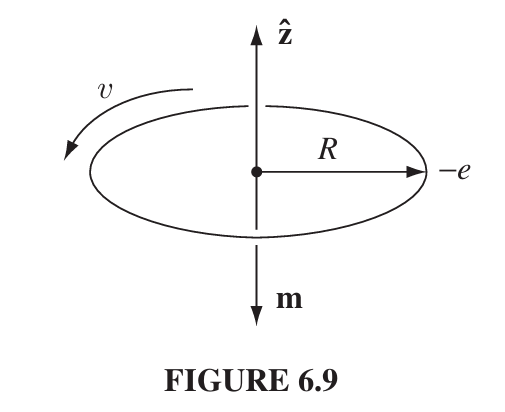
\includegraphics[width=0.7\textwidth]{IMG/fig69.png}
	\end{figure}
	
	\esp
	
	\begin{figure}[H]
		\centering
		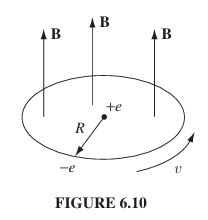
\includegraphics[width=0.7\textwidth]{IMG/fig610.png}
	\end{figure}
	
	\esp
	
	o, asumiendo que el cambio $\Delta v = \bar{v} - v$ es pequeño,
	
	\esp
	
	\begin{equation}
		\Delta v = \frac{eRB}{2m_e}. \tag{6.7}
	\end{equation}
	
	\esp
	
	Cuando se enciende el campo $\mathbf{B}$, el electrón se acelera.$^3$ 
	Un cambio en la velocidad orbital significa un cambio en el momento dipolar (Ec. 6.4):
	
	\esp
	
	\begin{equation}
		\Delta \mathbf{m} = -\frac{1}{2} e(\Delta v)R \mathbf{\hat{z}} = -\frac{e^2 R^2}{4m_e} \mathbf{B}. \tag{6.8}
	\end{equation}
	
	\esp
	
	Observe que \textit{el cambio en} $\mathbf{m}$ \textit{es opuesto a la dirección de} $\mathbf{B}$. (Un electrón girando en el otro sentido tendría un momento dipolar apuntando hacia arriba, pero dicha órbita se vería frenada por el campo, por lo que el \textit{cambio} sigue siendo opuesto a $\mathbf{B}$). Ordinariamente, las órbitas de los electrones están orientadas al azar y los momentos dipolares orbitales se cancelan entre sí. Pero en presencia de un campo magnético, cada átomo adquiere un pequeño momento dipolar ``extra'', y estos incrementos son todos \textit{antiparalelos} al campo. Este es el mecanismo responsable del \textbf{diamagnetismo}. Es un fenómeno universal que afecta a todos los átomos. Sin embargo, suele ser mucho más débil que el paramagnetismo y, por lo tanto, se observa principalmente en átomos con números \textit{pares} de electrones, donde el paramagnetismo suele estar ausente.
	
	\esp
	
	Al derivar la Ec. 6.8, asumí que la órbita permanece circular, con su radio original $R$. No puedo ofrecer una justificación para esto en esta etapa. Si el átomo está estacionario mientras se enciende el campo, entonces mi suposición puede demostrarse —esto no es \textit{magnetostática}, sin embargo, y los detalles deberán esperar al Capítulo 7 (ver Prob. 7.52). Si el átomo se mueve hacia el interior del campo, la situación es enormemente más complicada. Pero no importa; solo intento dar una explicación cualitativa del diamagnetismo. Asuma, si lo prefiere, que la velocidad permanece igual mientras el \textit{radio} cambia —la fórmula (Ec. 6.8) se ve alterada (por un factor de 2), pero la conclusión cualitativa no se ve afectada. La verdad es que este modelo clásico es fundamentalmente defectuoso (el diamagnetismo es en realidad un fenómeno \textit{cuántico}), por lo que no tiene mucho sentido refinar los detalles. Lo que \textit{es} importante es el hecho empírico de que en los materiales diamagnéticos los momentos dipolares inducidos apuntan en dirección opuesta al campo magnético.
	
	\printbibliography[title={Bibliografía}]
\end{document}